\begin{figure}[!ht]
\centering
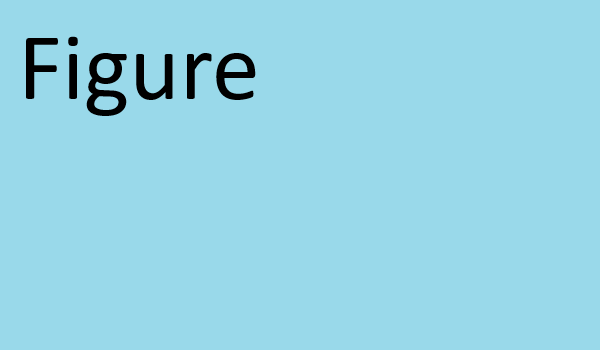
\includegraphics[width = 0.45\textwidth]{figure/place_holder.png}
\caption{Description.}
\label{fig:place_holder}
\end{figure}

\begin{table}[!ht]
    \centering
    \caption{Parameter values}
    \begin{tabular}{ ccccccc }
    \hline
    $\tau_{in}$ & $\tau_{out}$ & $\tau_{open}$ & $\tau_{close}$ & $u_{gate}$ \\\hline
    0.3 ms & 6 ms & 120 ms & 80 ms & 0.13 mV \\ 
    \hline
    \end{tabular}
    \label{tb:parameter}
    \begin{flushleft}
    Description
    \end{flushleft}
\end{table}

\begin{align}
\label{eq:mitchell schaeffer}
\begin{split}
\frac{du}{dt}&=\frac{hu^2(1-u)}{\tau _{in}}-\frac{u}{\tau _{out}}+J+\bigtriangledown \cdot (D\bigtriangledown u)
\\
\frac{dh}{dt}&=\left\{\begin{matrix}\ \frac{1-h}{\tau_{open}} \ \text{if}\ u<u_{gate} \\ \ \frac{-h}{\tau_{close}} \ \text{if}\ u \geq u_{gate}\end{matrix}\right.
\end{split}
\end{align}